\chapter{Algoritmos e tela LCD}
\section*{Introdução}
    Neste capítulo veremos o que significa algoritmo, o que é uma tela LCD e para que ela serve. Além disso, vamos abordar o conceito de linguagem de programação e saber, afinal, como nos comunicar com o \textit{Sparki}. E aí, vamos nessa?
\section{Algoritmo}
    Diariamente utilizamos algoritmos sem mesmo perceber. Quando cozinhamos um macarrão, assamos um bolo, montamos um móvel, um brinquedo ou mesmo quando escovamos os dentes estamos utilizando este conceito para completar essas tarefas. \par
    Isto porque tomamos essas decisões nos baseando em instruções claras para chegar a um objetivo. Então, se estamos preparando um bolo, não podemos simplesmente colocar os ingredientes no forno sem antes misturá-los conforme a receita. Não teríamos um bolo, mas um Frankestein! Da mesma forma, não poderíamos esperar que ele fique pronto se ligarmos o forno, mas não colocássemos a massa do bolo nele. \par
    \begin{center}
    \textbf{Definição} \\
    Algoritmo é um conjunto finito de instruções sequenciais lógicas, bem definidas, não ambíguas que levam à solução de um problema.
    \end{center}
    \textit{Mas afinal o que esse bando de palavras complicadas querem dizer ? Eu não entendi foi nada.}
    
    O que elas querem dizer é, em outras palavras, que um algoritmo indica um conjunto de instruções para realizar uma tarefa qualquer, como por exemplo, fazer pipoca. Seguimos uma receita que nos diz bem direitinho o que fazer para atingir o objetivo desejado, que no caso é aquela pipoca bem quentinha e crocante no final das contas! Assim ficou mais fácil de entender, né? \par
    Como já vimos, robôs não raciocinam como nós, seres humanos. Então precisamos deixar bem claro o que esperamos de cada um deles quando estamos nos comunicamos com eles para que o objetivo final seja cumprido. 
    
    \textit{Ué, mas isto parece exatamente com algo que você já disse.}  
    
    Exatamente! Escrevemos algoritmos para fazer a programação de robôs! \par 
    Até agora vimos que algoritmos são extremamente importantes e é essencial que o seu conceito seja entendido. Mas você sabia que não precisamos de um computador para programar?
\subsection{Torre de copos}
    \begin{figure}[h]
    \caption{Exemplo de um torre feita com copos}
     
    \centering 
    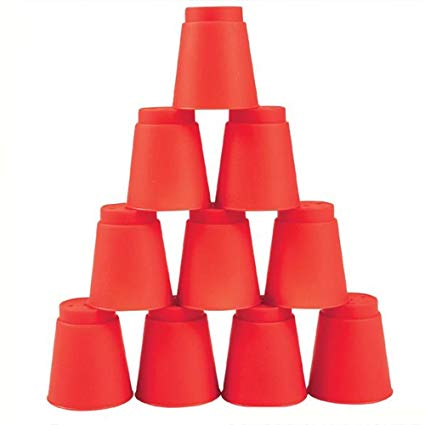
\includegraphics[width=8cm]{Figuras/torre.jpg}
    \label{figura:torre.jpeg}
    \end{figure}

Que tal vermos um exemplo de como você pode criar um algoritmo facilmente, tudo o que você precisa é de alguns copos de preferência de plástico e de algum lugar para escrever, você deve começar agora a criar instruções básicas necessárias para transformar uma pilha normal de copos na sua majestosa torre de copos, como "\textbf{pegar copo}", "\textbf{soltar copo}", "\textbf{mover o copo para cima, para a direita ou esquerda}" e outras que você julgar úteis desde que todas elas sejam bem simples e diretas (sem duplo sentido), você não pode simplesmente fazer a instrução "\textbf{monta torre}" ou "\textbf{vire de cabeça para baixo}", porque você não deixou claro se é para virar o copo de cabeça para baixo, ou a pessoa de cabeça para baixo, ou a cadeira, e etc.

Agora que você tem todo o seu conjunto de instruções, hora de organizá-las de forma sequencial para que você mesmo ou o seu amigo siga elas a fino, e assim seja capaz de no final ter uma torre de copos montada em sua frente.

Ex:"\textbf{pegar copo, mover copo para direita, soltar copo, mover a mão para esquerda, pegar copo...}"

Como o que você acabou de fazer é um conjunto finito de instruções bem definidas sem ambiguidade, simples e escritas de forma sequencial, onde tudo foi feito com o objetivo de realizarmos uma tarefa (montar a torre), podemos concluir então que o que você fez \textbf{É} um algoritmo.




\section{Linguagem de programação}
    Se fosse dado o comando abaixo para o \textit{Sparki} você acha que ele entenderia? \par
    \begin{center}
    \textit{Sparki vai para frente! Sparki vai para trás!}\ \par
    \end{center} \par
    Quem pensou que ele não entenderia acertou, o \textit{Sparki} não iria entender nada do que foi dito. \par
    \textit{Então como ele entende os comandos que pedimos para ele fazer?}\par
    Para nos comunicarmos com o \textit{Sparki}, é preciso passar os comandos para o computador através de uma linguagem de programação, que irá converter o que escrevemos para zeros e uns e depois enviará para \textit{Sparki}, e assim ele será capaz de entender e executar o comando.
    
    \begin{center}
    \textbf{Definição} \\
    Uma linguagem de programação é um método padronizado para comunicar instruções para um computador.
    \end{center} \par
    
De maneira mais simples, linguagem de programação é a língua que usamos para nos comunicar com o computador assim como a língua portuguesa é a língua que usamos para nos comunicar entre nós. Assim como existem várias línguas como inglês, alemão e japonês, existem várias linguagens de programação cada uma com suas peculiaridades, mas aqui no nosso curso iremos focar em aprender a linguagem que o \textit{Sparki} usa.

Como mencionado anteriormente, o que escrevermos para o \textit{Sparki} é antes transformados em 0's e 1's, isso porque os computadores utilizam a notação \textbf{binária}, onde os números são representados apenas utilizando-se de zeros e uns. Podemos concluir então que na verdade, os computadores não entendem a linguagem de programação!! Tudo o que escrevemos para eles em linguagem de programação é depois transformado em 0's e 1's para que finalmente possamos nos comunicar.
    
 
\subsection{Funções importantes: \textit{void setup(), void loop()}}
    
    A biblioteca  \textit{sparki.h} e as funções \textit{void setup e void loop} são as funções mais importantes na hora de começar a programar o \textit{Sparki}, pois entender o que elas significam e como funcionam é essencial para saber onde escrever determinada parte do código em relação ao tipo de aplicação.
    
    \begin{minted}{cpp}
    #include <Sparki.h>
    void setup()
    {
    }
    void loop()
    {
    }
    \end{minted}

    \begin{itemize}
        \item Biblioteca \textit{sparki.h}: Esta biblioteca guarda todas as funções relacionadas ao \textit{Sparki}, e é necessário inserir ela na primeira linha de código, para que estas funções sejam habilitadas para a comunicação entre o computador e o robô funcionar.
        \item \textit{Void Setup()}: Esta função é a primeira a rodar no código, e tudo que está dentro de suas chaves é executado apenas uma vez. A função é bastante útil para inserir configurações iniciais, como por exemplo limpar a tela LCD, ou fazer algum movimento inicial que não irá se repetir no resto do programa.
        \item \textit{Void Loop}: Esta função é usada para colocar códigos que irão ficar se repetindo no programa, ou seja, sempre ficará rodando até que seja carregado algum outro programa no \textit{Sparki}. Um exemplo para esta função é deixar o \textit{Sparki} sempre com o LED de uma cor ligado, ou sempre se movimentando em uma determinada direção.
        \end{itemize}
    
  %  Escrever código de como mostrar algo na tela do Sparki

\section{Tela de LCD (\textit{Liquid Crystal Display})}
O \textit{Sparki} possui uma tela LCD onde é possível desenhar, escrever e visualizar dados de sensores em funcionamento. A tela é formada por \textit{pixels}, que são pequenos pontos de luz que podem estar ligados ou desligados para formar uma imagem. No caso do \textit{Sparki}, ele possui 128 \textit{pixels} na horizontal e 64 \textit{pixels} na vertical, e para identificar cada pixel deve ser fornecido a coordenada horizontal, vertical, e se ele deverá ficar aceso ou apagado. \par
\textit{Então toda vez que eu for escrever algo no LCD preciso fazer a coordenada de cada pixel?}
Não, porque alguém já disse ao computador como ligar e desligar pixels para formar os caracteres, ou seja, se você quer escrever uma letra 'A' por exemplo, já está armazenado quais pixels devem acender e apagar para que a tela mostre exatamente a letra 'A'.

\section{Exercícios}
\question{Em suas palavras, defina o que é uma linguagem de programação.}
    Deixar espaço de linhas.
    \vspace{4cm}        % Espaçamento vertical
    
\question{O objetivo de uma linguagem de programação é:}
    \begin{enumerate}
        \item Fornecer um conjunto de regras bem definidas que permita escrever programas de computador de forma mais amigável evitando ambiguidades.
        \item Dar a liberdade para cada programador escrever programas de computador a partir do seu próprio conjunto de regras, facilitando o processo de programação.
        \item Estabelecer regras para comunicação entre seres humanos.
        \item Definir um padrão para programadores utilizarem os comandos binários intrínsecos a cada arquitetura de processador.
    \end{enumerate}

\subsection{}

\subsection{}

\subsection{}

\subsection{\large{Desafio:}}
% Capítulo Movimentação =========================================